% -*- root: ../main.tex -*-
%!TEX root = ../main.tex
% this file is called up by main.tex
% content in this file will be fed into the main document
% vim:textwidth=80 fo=cqt


The      transfer     function      identification     techniques      mentioned
in \cref{sec:introblackboxsysid} are  applicable only for \gls{lti}  systems. At
first glance,  this seems to  be overly restrictive  for the system(s)  at hand.
When  considered  as  a  single  macroscopic  entity,  a  lithium  ion  battery,
exhibits  overall non-linear  characteristics,  particularly due  to the  strong
non-linearities in
\begin{enumerate*}[label=\emph{\alph*})]
    \item the Butler-Volmer reaction kinetics (see \cref{eq:butlervolmer}), and
    \item the \glspl{ocp} of the two electrodes (see \cref{eq:lcoUocpPos} and \cref{eq:lcoUocpPos}).
\end{enumerate*}
However,  we are  dealing with  a much  narrower scope  \ie~the  systems under
consideration  are just  the two  sub-system entities  (one per  electrode) that
transform the  applied current at  a particular  time-step to the  overall moles
per  unit area  of  \ch{Li^+}  ions in  the  corresponding  electrode region  of
the  electrolyte at  that  same  instant. Therefore,  it  is  the linearity  and
time-invariance of these \emph{subsystems} that must be investigated.

\subsection{Time-invariance of the electrolyte time-evolution subsystems}\label{subsec:timeinvariance}
A  test  for time-invariance  is  prescribed  in  the  lecture notes  on  system
identification by  Plett~\cite{PlettECE5560_02}. The steps involved  therein are
reproduced here after  being suitably adapted to the notation  of the subsystems
at hand.
\begin{enumerate}
    \item Apply input $u_1(t) = I(t)$ to the system and measure the outputs $Q_{\text{e,n}_1}\!(t)$ and $Q_{\text{e,p}_1}\!(t)$.
    \item Apply a delayed version of the input by $\tau$ seconds \ie~$u_2(t) = I(t-\tau)$ to the system and measure the outputs $Q_{\text{e,n}_2}\!(t)$ and $Q_{\text{e,n}_2}\!(t)$.
    \item If $Q_{\text{e,n}_2}\!(t)$ = $Q_{\text{e,n}_1}\!(t-\tau)$ and
        $Q_{\text{e,p}_2}\!(t)$ = $Q_{\text{e,p}_1}\!(t-\tau)$ for all possible
        delays $\tau$, as well as for all choice of input signals $I(t)$, then the systems are time-invariant.
\end{enumerate}

For the systems at hand, it is  not strictly required to apply this prescriptive
test. Unless a fundamental change in the underlying reaction phenomena/chemistry
occur that  alter the  performance over  time, these systems  can be  treated as
time-invariant. Factors  that induce  time-dependent shift  in the  behaviour of
lithium ion batteries are degradation  phenomena such as thickening of \gls{sei}
layer, dendrite growth or mechanical  fatigue in electrodes which in-turn affect
electrolytic  diffusion and  conductivity. Yet  another cause  of time-dependent
behavioural change  is the drift  in parameter values. However,  these phenomena
are  typically  one or  mode  orders  of  magnitude  slower than  the  \gls{p2d}
dynamics\fxnote{citation needed}. This separation  of time-scales imply that, in
practice they can be decoupled. Therefore, separate models can be identified for
the faster and slower processes. A  suitable model-blending approach can then be
considered  to cover  all processes  across time-scales.  Although the  concepts
developed here for the fast electrolyte dynamics can be suitably adapted to such
slow phenomena, their study  falls outside the scope of this  thesis and is left
as an exercise for  future work. Thus, the overall battery  system, and hence by
extension,  the  two subsystems  considered  are  deemed to  be  time-invariant.
However, in the interest of completeness, this author systematically applied the
aforementioned test procedure with every  combination arising from the choice of
ten time-delay values and the following six current profiles ---
\begin{enumerate*}[label=\emph{\alph*})]
    \item constant current 1C discharge,
    \item constant current 3C discharge,
    \item constant current 1C charge,
    \item \gls{udds} input profile with peak amplitude of 3C,
    \item training profile used in system identification (see \cref{fig:sysidtrainingcurrent}), and
    \item validation profile used in system identification (see \cref{fig:sysidvalidationcurrent}).
\end{enumerate*}
Finally,  these tests  were  repeated for  a choice  of  five different  initial
\glspl{soc}   ---   \SI{90}{\percent},   \SI{70}{\percent},   \SI{50}{\percent},
\SI{30}{\percent}  and \SI{10}{\percent}\footnote{\label{fn:socstart}The  number
of  moles  of  \ch{Li^+} per  unit  area  in  the  electrolyte does  not  depend
on  the  electrode's \glsfmtshort{soc}.  However,  different  starting point  of
\glsfmtshort{soc}s were considered  to have a wide variety in  the length of the
recorded  data until  cut-offs  were hit.  \eg~starting at  \SI{90}{\percent}
\glsfmtshort{soc} could  mean that  for a  current spike  early in  the profile,
upper  cut-off voltage  shall be  hit  sooner leaving  a smaller  set of  logged
simulation data.}.

\begin{figure}[!htbp]
    \centering
    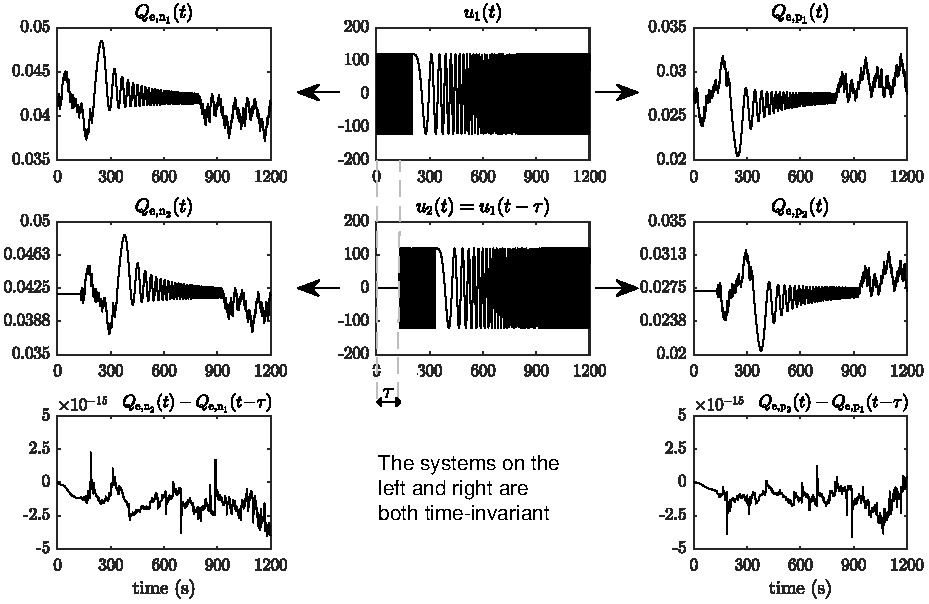
\includegraphics[width=\textwidth]{time_invariance.pdf}
    \caption[Demonstration of time-invariance of $Q_\text{e,n}(t)$ and
    $Q_\text{e,p}(t)$ subsystems]{Demonstration of time-invariance of the
        subsystems considered. The applied current profile $u_1(t)$ is the
        system identification training sequence
        from \cref{fig:sysidtrainingcurrent} (top row of the central column).
        The top left plot shows the response $Q_{\text{e,n}_1}\!(t)$, while that
        on the top right shows $Q_{\text{e,p}_1}\!(t)$. The second row of the
        middle column shows the same input sequence delayed by $\tau =
        \SI{130}{\second}$. Application of this current profile $u_2(t) =
        u_1(t-\tau)$ results in the outputs $Q_{\text{e,n}_2}\!(t)$ and
        $Q_{\text{e,p}_2}\!(t)$ to its left and right respectively. Subtracting
        these from the correspondingly delayed versions of the original outputs
        result in zero residuals, thereby proving time-invariance of these
        subsystems. The jitter shown in the bottom row of plots is
        $\mathcal{O}(10^{-15})$ in magnitude and are due to the numerical
        roundoffs that occur when operating close to the noise floor of the
    machine's floating point units.}%
\label{fig:timeinvariance}
\end{figure}
% The outputs $Q_\text{e,n}$ and $Q_\text{e,p}$ are shown to the left and right of the applied input.

\Cref{fig:timeinvariance}  demonstrates the  time-invariance  of the  subsystems
considered  at  an  initial  \gls{soc} of  \SI{50}{\percent}  for  a  time-delay
of   \SI{130}{\second}   using   the  highly   dynamic   system   identification
training    sequence   that    was   synthesised    by   this    thesis   author
(see \cref{fig:sysidtrainingcurrent}).  The  applied  current  profile  $u_1(t)$
(top row  of the  central column)  produces the  outputs $Q_{\text{e,n}_1}\!(t)$
and  $Q_{\text{e,p}_1}\!(t)$  shown  in  the   top  left  and  top  right  plots
respectively.  When  the delayed  version  of  this  input sequence  ${u_2(t)  =
u_1(t-\tau)}$ (middle row, middle column) is  applied, it results in the outputs
$Q_{\text{e,n}_2}\!(t)$  and  $Q_{\text{e,p}_2}\!(t)$  to  its  left  and  right
respectively.  Following the  steps  of the  test  procedure, subtracting  these
outputs from the correspondingly delayed versions of their original counterparts
result in  zero residuals, thereby  proving time-invariance of  these subsystems
under these representative test conditions. The residual sequences in the bottom
row of plots are of $\mathcal{O}(10^{-15})$ and arise due to numerical roundoffs
that occur  when operating close  to the noise  floor of the  machine's floating
point units.

Similar to  the case demonstrated  here, all  tests for time-invariance  for all
permutations of  the chosen operating  conditions passed successfully  \ie~the
delayed  version of  the original  output  signals accurately  matched with  the
responses  to  the corresponding  delayed  input  (down to  machine  precision),
thereby confirming the time-variance of  the subsystems considered in the system
identification problem, which enables us to proceed further.


\subsection{Linearity analysis of the electrolyte time-evolution subsystems}\label{subsec:linearityanalysis}

\subsubsection*{De-biasing of  input signals}
In the analyses of linearity of systems, it is a recommended practice to de-bias
the output and input quantities about their mean operating conditions. The input
signal  in this  case is  the applied  load current  $I(t)$, which  can be  both
positive  (during discharge)  and  negative  (during charge).  The  mean of  the
training profile is  \SI{-1.167}{\ampere} and that of the  validation profile is
\SI{-0.3273}{\ampere}. Clearly,  the mean values  are dependent upon  the actual
current profile used. The appropriately de-biased signal \ie~$\widetilde{I}(t)
= I(t) - \bar{I}(t)$ is to be used  for training and validation data sets in the
system identification procedure. For the purpose  of linearity analysis, it is a
standard practice to simply apply a step change in input (from zero) and measure
the output responses, thereby bypassing the de-biasing requirements.

% Although, in  principle, the strength  of the input  signal does not  affect the
% linearity tests, for  the actual system identification  procedure, the de-biased
% signal must still be persistently exciting as in \cref{sec:persistentexcitation}
% must be

For the output signals, bias  values can be pre-computed analytically and
accounted for.  The overall number  of moles of \ch{Li^+}  per unit area  in any
region within  the cell cannot  be physically  negative. Even though  under high
C-rates,  ion depletion  at localised  spatial  locations (such  as the  current
collectors) is  certainly possible,  the entire thickness  of any  region cannot
become devoid of ions at any point  in time since the cell shall instantaneously
cease  to work.  Thus, for  a typical  well-designed cell  operating within  the
manufacturer prescribed  C-rate limits,  the output signals  under consideration
operate  in  a  small  window  about  their  initial  values.  In  the  author's
simulations, even  at $\pm$5C, the overall  number of moles of  \ch{Li^+} in any
cell region exhibited  a maximum change of less than  \SI{15}{\percent} from its
initial value. Thus,  the de-biased output variables  for system identification,
$\widetilde{Q}_{\text{e,}j}(t)$ can be obtained  by subtracting their respective
initial values $Q_{\text{e,}j}(0)$ (see \cref{eq:Qeninit} and \cref{eq:Qepinit})
from $Q_{\text{e,}j}(t)$.
\begin{align}
    \widetilde{Q}_\text{e,n}(t) & = {Q}_\text{e,n}(t) - {Q}_\text{e,n}(0) \\
    \widetilde{Q}_\text{e,p}(t) & = {Q}_\text{e,p}(t) - {Q}_\text{e,p}(0)
\end{align}
which  implies   that  the   transfer  functions  to   be  identified   have  to
be   modified   to   be   $\frac{\widetilde{Q}_\text{e,n}(s)}{\bar{I}(s)}$   and
$\frac{\widetilde{Q}_\text{e,p}(s)}{\bar{I}(s)}$  respectively.  This  does  not
affect  the  time-invariance  proved in \cref{subsec:timeinvariance}  since  the
initial  values   $Q_{\text{e,}j}(0)$  are   merely  constants  and   hence  not
time-dependent.

\subsubsection*{Test for linearity}
Similar     to      the     test      for     time      invariance     described
in \cref{subsec:timeinvariance}, a  test for linearity is  also prescribed in
the lecture notes on  system identification by Plett~\cite{PlettECE5560_02}. The
steps involved therein  are reproduced here after being suitably  adapted to the
notation of the subsystems at hand. This is essentially a recipe for testing the
superposition principle.
\begin{enumerate}
    \item Apply input profile $I_1(t)$ to the system and obtain outputs $\widetilde{Q}_{\text{e,n}_1}\!(t)$ and $\widetilde{Q}_{\text{e,p}_1}\!(t)$.
    \item Apply a different profile $I_2(t)$ to the system and obtain outputs $\widetilde{Q}_{\text{e,n}_2}\!(t)$ and $\widetilde{Q}_{\text{e,n}_2}\!(t)$.
    \item Now apply an input profile $I_3(t) = \alpha I_1(t) + \beta I_2(t)$ and obtain a corresponding set of outputs $\widetilde{Q}_{\text{e,n}_3}\!(t)$ and $\widetilde{Q}_{\text{e,n}_3}\!(t)$.
    \item If $\widetilde{Q}_{\text{e,n}_3}\!(t)$ = $\alpha\, \widetilde{Q}_{\text{e,n}_1}\!(t) + \beta \, \widetilde{Q}_{\text{e,n}_2}\!(t)$ and $\widetilde{Q}_{\text{e,p}_3}\!(t)$ = $\alpha\, \widetilde{Q}_{\text{e,p}_1}\!(t) + \beta \, \widetilde{Q}_{\text{e,p}_2}\!(t)$ for all possible $\{\alpha,\beta\}$ as well as for choice of input signals $\{I_1(t),I_2(t)\}$, then the systems are linear.
\end{enumerate}

As   in   the  time-invariance   test,   the   same   set  of   five   different
initial  \glspl{soc}\textsuperscript{\ref{fn:socstart}}  ---  \SI{90}{\percent},
\SI{70}{\percent},  \SI{50}{\percent}, \SI{30}{\percent}  and \SI{10}{\percent},
was  retained for  these linearity  tests. For  each test  run, a  pseudo-random
number generator  was used to select  the values of $\{\alpha,\beta\}$  from the
set  of  real numbers  $\mathbb{R}$  (not  restricted  to  the set  of  integers
$\mathbb{Z}$) in  the closed  interval spanning $[-1.25,1.25]$.  Negative values
are acceptable for  both the scaling coefficients since  the resulting composite
input $I_3(t)$ can be either positive or negative. The composite signal $I_3(t)$
was obtained by taking a random combination  of any two of the following current
profiles ---
\begin{enumerate*}[label=\emph{\alph*})]
    \item step input with a constant current 1C discharge,
    \item step input with a constant current discharge at C/5,
    \item step input with a constant current 1C charge,
    \item step input with a constant current charge at C/5,
    % \item de-biased training profile used in system identification (see \cref{fig:sysidtrainingcurrent}), and
    % \item de-biased validation profile used in system identification (see \cref{fig:sysidvalidationcurrent}).
\end{enumerate*}

The  scaling  factors  $\alpha$  and   $\beta$  were  restricted  to  the  range
$[-1.25,1.25]$ in consideration of limiting the peak applied current to within a
\pm 3C  window ---  the operating  condition for most  \glspl{bev}, so  that the
isothermal assumption for the model shall remain valid. This peak current corner
case occurs when the pseudo-random generator chooses both scaling factors at the
selected range's limits for the 1C constant current discharge or charging cases.
The limited  range of the  scaling factors are also  motivated by the  fact that
most real-world systems remain linear only within a certain operating window. In
particular, care  must be taken to  ensure that the cell's  \gls{soc} during the
linearity test  remains within  its physical limits  for any  initial \gls{soc}.
Furthermore, localised  saturation or depletion  of ions for  extended durations
must be avoided. Hence  it can be concluded that, with the  chosen range for the
scaling  factors,  if  the  two subsystems  under  consideration  remain  linear
everywhere below  a peak  current of  \pm 3C  in the  isothermal case,  then the
linearity  tests are  considered as  passed.  Future extensions  to undertake  a
temperature-dependent  system  identification  exercise can  potentially  use  a
first-order Taylor  expansion about this  operating window. The  discussion thus
far  has fully  established  all  the conditions  for  conducting  the test  for
linearity.

\begin{figure}[!htbp]
    \centering
    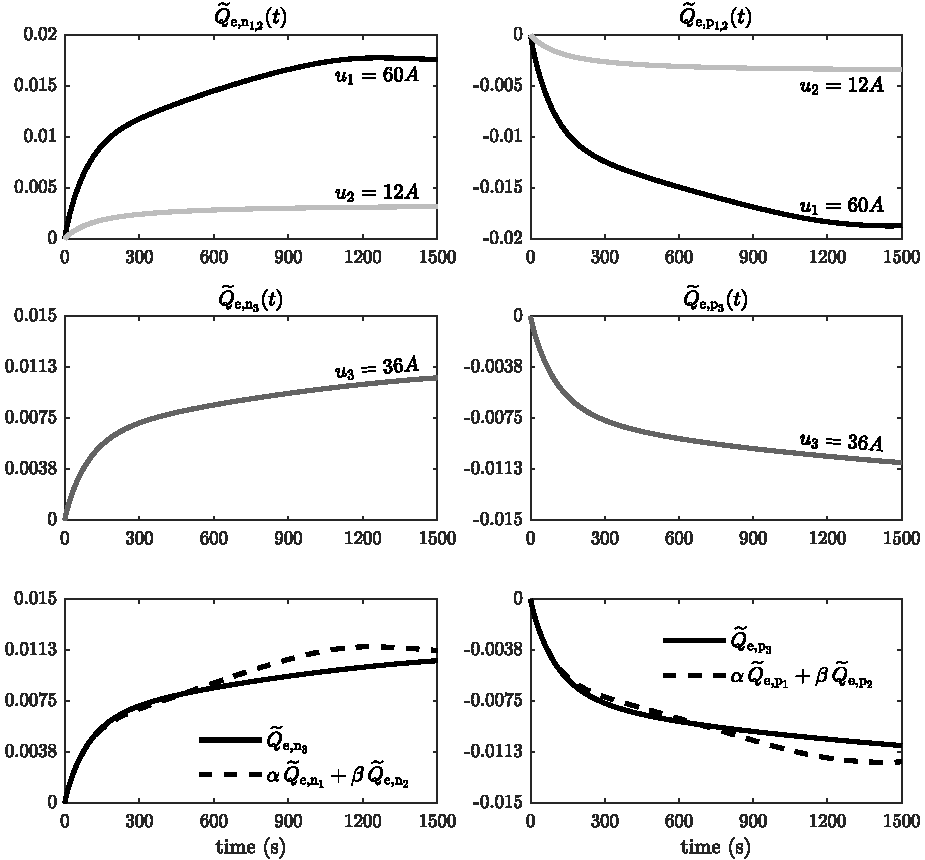
\includegraphics[width=\textwidth]{linearity_proof}
    \caption[Illustration of linearity test for the
    \protect{$\widetilde{Q}_{\text{e,n}}$} and
    \protect{$\widetilde{Q}_{\text{e,p}}$} subsystems]{Illustration of one
        instance of linearity tests for the subsystems under consideration. For
        this visualisation, constant current inputs are used throughout. The top
        row of plots shows $\widetilde{Q}_{\text{e,n}}$ and
        $\widetilde{Q}_{\text{e,p}}$ for two step inputs $I_1(t) =
        \SI{60}{\ampere}$ and $I_2(t) = \SI{12}{\ampere}$ \ie~discharge with
        1C and C/5 currents respectively. The second row of plots shows
        $\widetilde{Q}_{\text{e,n}_3}$ and $\widetilde{Q}_{\text{e,p}_3}$  for
        $I_3 = \SI{36}{\ampere}$, where $I_3 = \alpha I_1 + \beta I_2$ with
        $(\alpha,\beta) = (1,-2)$. The last row of plots overlays these
        quantities with the manually computed linear combination of their two
        preceding responses. Had these sequences overlapped exactly, the systems
        would have been exactly linear. Despite exhibiting deviations over the
        considered horizon, the transient responses in both electrode regions do
        follow the superposition principle. Even past the transient, maximum
        error in both cases is an order of magnitude lower than the individual
        outputs. Hence, the two systems are deemed to be \emph{approximately}
        linear.
    }%
    \label{fig:linearity}
\end{figure}

\Cref{fig:linearity}  illustrates  one  instance  of a  linearity  test  wherein
constant  currents  and  integer  scaling  factors are  used  for  the  sake  of
illustration.  The  plots   in  the  left  column  deal   with  the  electrolyte
time-evolution  subsystem  in  the  negative electrode  region.  Similarly,  the
plots  in  the  right  column  deal with  the  corresponding  subsystem  in  the
positive electrode region.  A discharge current of 1C  \ie~\SI{60}{\ampere} is
first  applied  and  the  corresponding  outputs  $\widetilde{Q}_{\text{e,n}_1}$
and   $\widetilde{Q}_{\text{e,p}_1}$  are   obtained.   Secondly,  a   discharge
current   of   C/5   \ie~is    applied   and   the   corresponding   outputs
$\widetilde{Q}_{\text{e,n}_2}$ and  $\widetilde{Q}_{\text{e,p}_2}$ are obtained.
These set of responses are plotted  in the top row of \cref{fig:linearity}. Now,
a  third  value  of  input  current $I_3$,  computed  as  a  linear  combination
of  the  previous  input  currents  \ie~$I_3 =  \alpha  I_1  +  \beta  I_2  $
is  applied.  For  illustrative  purposes, the  integer  set  $(\alpha,\beta)  =
(1,-2)$  was  chosen  for  the   scaling  coefficients,  which  implies  $I_3  =
\SI{12}{\ampere}$. The corresponding  outputs $\widetilde{Q}_{\text{e,n}_3}$ and
$\widetilde{Q}_{\text{e,p}_3}$ are  plotted in the  middle row. As per  the test
for linearity,  if these signals are  equal to the signal  generated by manually
computing the linear  combination of the preceding two outputs,  then the system
is linear.

The   plots   in  the   third   row   show  $\widetilde{Q}_{\text{e,n}_3}$   and
$\widetilde{Q}_{\text{e,p}_3}$ overlaid with their respective linear combination
signals. In  the case  of the  subsystem in the  negative electrode  region, the
transient performance matches  precisely until \approx\SI{450}{\second}, whereas
that in the positive electrode region exhibits a good matching for approximately
the  first  \SI{250}{\second}.  However,  for the  horizon  considered  the  two
overlaid plots do not overlap exactly.  Hence, the systems are not truly linear.
However, the exhibited  behaviour is quite close to linearity,  with the maximum
absolute  error  in each  region,  even  outside  the initial  transient,  being
$\mathcal{O}(10^{-4})$  --- an  order  of magnitude  lower  than its  individual
components.  This behaviour  was exhibited  for all  test instances  considered.
Considering  that for  dynamic  simulation runs,  the  transient performance  is
paramount  to  the good  performance  of  the  model,  in conjunction  with  the
aforementioned  low error  metric,  these  subsystems can  be  considered to  be
\emph{approximately} linear.

Based  on  the  analysis  presented   here,  \gls{lti}  behaviour  for  the  two
subsystems is  assumed, which facilitates  in proceeding with the  actual system
identification procedure.


